\documentclass[xcolor=table,aspectratio=169]{beamer}
\usetheme{Madrid}
\beamertemplatenavigationsymbolsempty
\usepackage{graphicx}
\usepackage[table]{xcolor}
\usepackage[most, skins]{tcolorbox}
\usepackage{helvet}
% Definitions of colours used in seaborn for use in latex
\definecolor{seaborn_bg_grey}{HTML}{eaeaf2}
\definecolor{seaborn_bg_grey_dark}{HTML}{d2d2d9}
\definecolor{seaborn_bg_grey_darker}{HTML}{a3a3a9}
\definecolor{seaborn_bg_grey_half}{HTML}{f4f4f8}

\definecolor{seaborn_blue}{HTML}{4c72b0}
\definecolor{seaborn_green}{HTML}{55a868}
\definecolor{seaborn_red}{HTML}{c44e52}
\definecolor{seaborn_magenta}{HTML}{8172b2}
\definecolor{seaborn_yellow}{HTML}{ccb974}
\definecolor{seaborn_cyan}{HTML}{64b5cd}

\definecolor{seaborn_muted_blue}{HTML}{4878cf}
\definecolor{seaborn_muted_green}{HTML}{6acc65}
\definecolor{seaborn_muted_red}{HTML}{d65f5f}
\definecolor{seaborn_muted_magenta}{HTML}{b47cc7}
\definecolor{seaborn_muted_yellow}{HTML}{c4ad66}
\definecolor{seaborn_muted_cyan}{HTML}{77bedb}

\definecolor{seaborn_pastel_blue}{HTML}{92c6ff}
\definecolor{seaborn_pastel_green}{HTML}{97f0aa}
\definecolor{seaborn_pastel_red}{HTML}{ff9f9a}
\definecolor{seaborn_pastel_magenta}{HTML}{d0bbff}
\definecolor{seaborn_pastel_yellow}{HTML}{fffea3}
\definecolor{seaborn_pastel_cyan}{HTML}{b0e0e6}

\definecolor{seaborn_bright_blue}{HTML}{003fff}
\definecolor{seaborn_bright_green}{HTML}{03ed3a}
\definecolor{seaborn_bright_red}{HTML}{e8000b}
\definecolor{seaborn_bright_magenta}{HTML}{8a2be2}
\definecolor{seaborn_bright_yellow}{HTML}{ffc400}
\definecolor{seaborn_bright_cyan}{HTML}{00d7ff}

\definecolor{seaborn_dark_blue}{HTML}{001c7f}
\definecolor{seaborn_dark_green}{HTML}{017517}
\definecolor{seaborn_dark_red}{HTML}{8c0900}
\definecolor{seaborn_dark_magenta}{HTML}{7600a1}
\definecolor{seaborn_dark_yellow}{HTML}{b8860b}
\definecolor{seaborn_dark_cyan}{HTML}{006374}

\definecolor{seaborn_colorblind_blue}{HTML}{0072b2}
\definecolor{seaborn_colorblind_green}{HTML}{009e73}
\definecolor{seaborn_colorblind_red}{HTML}{d55e00}
\definecolor{seaborn_colorblind_magenta}{HTML}{cc79a7}
\definecolor{seaborn_colorblind_yellow}{HTML}{f0e442}
\definecolor{seaborn_colorblind_cyan}{HTML}{56b4e9}


\usepackage{adjustbox}

% Tikz
\usepackage{tikz}
\usetikzlibrary{positioning,shapes,arrows,backgrounds,fit,calc,external}
\tikzexternalize
\tikzstyle{dummy} = []
\tikzstyle{line} = [draw, thick, -latex']
\tikzstyle{headless_line} = [draw, thick, -]
\tikzstyle{default}    = [rectangle, text centered, rounded corners, text=black, font=\sffamily\footnotesize, align=center]
\tikzstyle{default_text}    = [rectangle, text width=10cm, text=black,anchor=north west, font=\sffamily]
\tikzstyle{boxwhite} = [default, fill=white, rounded corners=0.1cm]
\tikzstyle{cp}    = [default, fill=seaborn_blue, text=white, text width=2.8cm, minimum height=0.5cm]
\tikzstyle{pw}    = [cp, fill=seaborn_green]
\tikzstyle{wannier90}    = [cp, fill=seaborn_cyan]
\tikzstyle{bespoke}    = [cp, fill=seaborn_magenta]
\tikzstyle{kcw}    = [cp, fill=seaborn_magenta]
\tikzstyle{observable}    = [cp, fill=seaborn_red]
\tikzset{
  -|-/.style={
    to path={
      (\tikztostart) -| ($(\tikztostart)!#1!(\tikztotarget)$) |- (\tikztotarget)
      \tikztonodes
    }
  },
  -|-/.default=0.5,
  |-|/.style={
    to path={
      (\tikztostart) |- ($(\tikztostart)!#1!(\tikztotarget)$) -| (\tikztotarget)
      \tikztonodes
    }
  },
  |-|/.default=0.5,
}

\newlength{\myyshift}
\setlength{\myyshift}{0.05cm}

\definecolor{darkblue}{HTML}{315472}
\setbeamercolor{frametitle}{bg=black, fg=white}
\setbeamercolor{body}{fg=black, bg=white}
\setbeamercolor*{author in head/foot}{bg=darkblue}
\setbeamercolor*{logo in head/foot}{bg=darkblue,fg=white}
\setbeamercolor*{title in head/foot}{bg=darkblue,fg=white}
\setbeamercolor*{date in head/foot}{bg=darkblue,fg=white}
\setbeamercolor{title}{bg=darkblue}
\setbeamercolor{footline}{bg=darkblue}
\setbeamercolor{caption name}{fg=darkblue}
\setbeamersize{text margin left=0.07cm,text margin right=0.07cm}
\setbeamercolor{background canvas}{bg=seaborn_bg_grey_dark}

% New commands
\newcommand{\ket}[1]{|#1\rangle}
\newcommand{\bra}[1]{\langle #1|}
\newcommand{\braket}[2]{\langle #1|#2\rangle}
\newcommand{\braopket}[3]{\langle #1|#2|#3\rangle}
\newcommand{\nline}{\nonumber \\}
\newcommand{\Trace}{\mathrm{Tr}}

\setbeamertemplate{frametitle}
{
  \vspace{-1pt}
  \begin{beamercolorbox}[wd=\paperwidth,ht=0.8cm]{frametitle}
    \hspace{0.05em}
    \begin{minipage}{0.85\textwidth}
      \small \bf
      Accurately predicting electron affinities with Koopmans spectral functionals

      \tiny
      Edward Linscott, Nicola Colonna, Riccardo De Gennaro, and Nicola Marzari
    \end{minipage}
    \hfill
    \begin{minipage}{0.1\textwidth}
    \includegraphics[height=0.55cm]{/home/elinscott/Pictures/epfl_logos/white_cropped.eps}
    \end{minipage}
    \hspace{0.2cm}
    \vspace{0.125cm}
  \end{beamercolorbox}%
}
\setbeamertemplate{title page}
{
}
%\setbeamerfont{frametitle}{series=\bfseries}
\setbeamertemplate{footline}{}

\begin{document}
\begin{frame}
        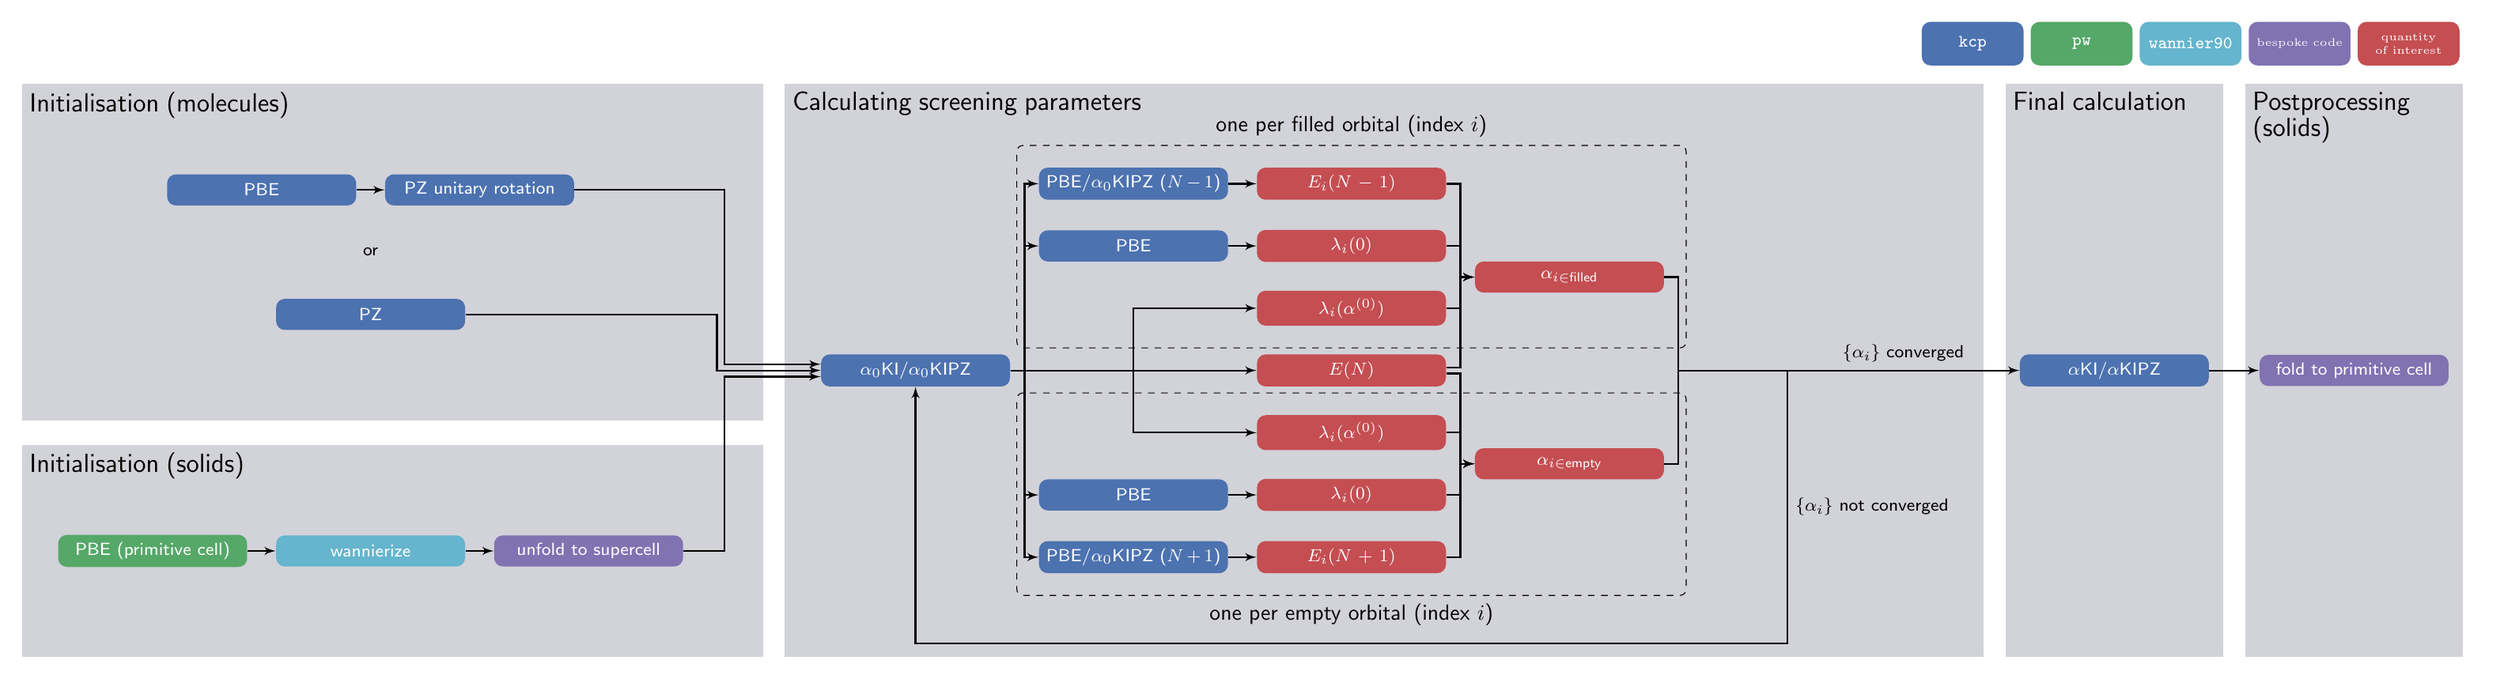
\begin{tikzpicture}[font=\tiny, x=3.5cm, y=1cm]
   \begin{pgfonlayer}{background}
      % \node[fit= (KC init) (empty label) (filled label) (sc loop 1) (converged label), fill=seaborn_bg_grey, inner sep=0.5cm] (calculating screening) {};
      % \node [dummy, above=0cm of calculating screening, font=\sffamily]{Calculating screening parameters};
      \fill [seaborn_bg_grey_dark] (-2.1,-0.8) rectangle (1.3,4.6);
      \node at (-2.1, 4.6) [default_text] {\large Initialisation (molecules)};
      \fill [seaborn_bg_grey_dark] (-2.1,-4.6) rectangle (1.3,-1.2);
      \node at (-2.1, -1.2) [default_text] {\large Initialisation (solids)};
      \fill [seaborn_bg_grey_dark] (1.4,-4.6) rectangle (6.9,4.6);
      \node at (1.4, 4.6) [default_text] {\large Calculating screening parameters};
      \fill [seaborn_bg_grey_dark] (7,-4.6) rectangle (8,4.6);
      \node at (7, 4.6) [default_text, text width=3.5cm] {\large Final calculation};
      \fill [seaborn_bg_grey_dark] (8.1,-4.6) rectangle (9.1,4.6);
      \node at (8.1, 4.6) [default_text, text width=3.5cm] {\large Postprocessing (solids)};
   \end{pgfonlayer}

   % Key
   \node at (6.85, 5.25) [cp, text width=1.4cm, minimum height=0.7cm] {\texttt{kcp}};
   \node at (7.35, 5.25) [pw, text width=1.4cm, minimum height=0.7cm] {\texttt{pw}};
   \node at (7.85, 5.25) [wannier90, text width=1.4cm, minimum height=0.7cm] {\texttt{wannier90}};
   \node at (8.35, 5.25) [bespoke, text width=1.4cm, minimum height=0.7cm, font=\tiny] {bespoke code};
   \node at (8.85, 5.25) [observable, text width=1.4cm, minimum height=0.7cm, font=\tiny] {quantity of interest};

   % Initialisation
   % Option 1
   \node at (-1, 2.9) [cp] (PBE init) {PBE};
   \node at (0, 2.9) [cp] (PZ innerloop) {PZ unitary rotation};
   \path [line] (PBE init) -- (PZ innerloop);

   % OR
   \node at (-0.5, 1.9) [default] (or) {or};

   % Option 2
   \node at (-0.5, 0.9) [cp] (PZ init) {PZ};

   % Solids
   \node at (-1.5, -2.9) [pw] (pw PBE init) {PBE (primitive cell)};
   \node at (-0.5, -2.9) [wannier90] (wannierize) {wannierize};
   \node at (0.5, -2.9) [bespoke] (unfold) {unfold to supercell};
   \path [line] (pw PBE init) -- (wannierize);
   \path [line] (wannierize) -- (unfold);

   % Calculating screening parameters
   \node at (2, 0) [cp] (KC init) {$\alpha_0$KI/$\alpha_0$KIPZ};

   \path let
   \p1 = (PZ innerloop),
   \p2 = (unfold.east)
   in
   coordinate (dummy) at (\x2, \y1);
   \path let
   \p1 = (PZ init),
   \p2 = (unfold.east)
   in
   coordinate (dummy2) at (\x2, \y1);
   \path [line] (PZ innerloop) -- (dummy) to[-|-=0.3] ([yshift=2\myyshift]KC init.west);
   \path [line] (PZ init.east) -- ([xshift=-3.5\myyshift]dummy2) to[-|-=0.3] (KC init.west);
   \path [line] (unfold.east) to[-|-=0.3] ([yshift=-2\myyshift]KC init.west);

   % KI filled %%%%%%%%%%%%%%%%%%%%%%%%%%%%%%%%%%%%%%%%%%%%%%%%%%

   % calculations
   \node at (3, 3) [cp] (N-1_filled) {PBE/$\alpha_0$KIPZ ($N-1$)};
   \node at (3, 2) [cp] (PBE_filled) {PBE};
   \node at (3, -2) [cp] (PBE_empty) {PBE};
   \node at (3, -3) [cp] (N+1_empty) {PBE/$\alpha_0$KIPZ ($N+1$)};

   \path [line] (KC init) to[-|-] (PBE_filled);
   \path [line] (KC init) to[-|-] (N-1_filled);
   \path [line] (KC init) to[-|-] (PBE_empty);
   \path [line] (KC init) to[-|-] (N+1_empty);

   % results
   \node at (4, 3) [observable] (EN-1_filled) {$E_i(N-1)$};
   \node at (4, 2) [observable] (lambda0_filled) {$\lambda_i(0)$};
   \node at (4, 1) [observable] (lambda_filled) {$\lambda_i(\alpha^{(0)})$};
   \node at (4, 0) [observable] (EN) {$E(N)$};
   \node at (4, -1) [observable] (lambda_empty) {$\lambda_i(\alpha^{(0)})$};
   \node at (4, -2) [observable] (lambda0_empty) {$\lambda_i(0)$};
   \node at (4, -3) [observable] (EN+1_empty) {$E_i(N+1)$};

   \path [line] (KC init) -- (EN);
   \path [line] (KC init.east) to[-|-] (lambda_filled.west);
   \path [line] (KC init.east) to[-|-] (lambda_empty.west);

   \path [line] (PBE_filled) -- (lambda0_filled);
   \path [line] (N-1_filled) -- (EN-1_filled);

   \path [line] (PBE_empty) -- (lambda0_empty);
   \path [line] (N+1_empty) -- (EN+1_empty);

   % alpha parameters
   \node at (5, 1.5) [observable] (alpha filled) {$\alpha_{i \in \text{filled}}$};
   \node at (5, -1.5) [observable] (alpha empty) {$\alpha_{i \in \text{empty}}$};

   \path [line] (lambda_filled) to[-|-] (alpha filled);
   \path [line] ([yshift=\myyshift]EN.east) to[-|-] (alpha filled.west);
   \path [line] (lambda0_filled) to[-|-] (alpha filled);
   \path [line] (EN-1_filled) to[-|-] (alpha filled);

   \path [line] (lambda_empty) to[-|-] (alpha empty);
   \path [line] ([yshift=-\myyshift]EN.east) to[-|-] (alpha empty.west);
   \path [line] (lambda0_empty) to[-|-] (alpha empty);
   \path [line] (EN+1_empty) to[-|-] (alpha empty);

   % SC check
   \coordinate (sc check) at (6, 0);
   \path [headless_line] (alpha empty) to[-|-] (sc check);
   \path [headless_line] (alpha filled) to[-|-] (sc check);

   % SC loop
   \node [below= of EN+1_empty] (sc loop y) {};
   \path let
   \p1 = (sc check),
   \p2 = (sc loop y)
   in
   coordinate (sc loop 1) at (\x1, \y2);
   \path [line] (sc check) -- node [midway, right, font=\sffamily] (not converged label) {\footnotesize $\{\alpha_i\}$ not converged} (sc loop 1) -| (KC init.south);

   % Final calc
   \node at (7.5, 0) [cp] (final KI) {$\alpha$KI/$\alpha$KIPZ};
   \path [line] (sc check) -- node [midway, above, font=\sffamily] (converged label) {\footnotesize $\{\alpha_i\}$ converged} (final KI);

   % Postproc
   \node at (8.6, 0) [bespoke] (upfold) {fold to primitive cell};
   \path [line] (final KI) -- (upfold);

   % Boxes
   % Screening parametere
   \node [boxwhite, fit= (N-1_filled) (lambda_filled) (alpha filled),
      draw, dashed, fill opacity=0, inner sep=0.35cm](filled box){};
   \node [dummy, above=0cm of filled box, font=\sffamily](filled label){one per filled orbital (index $i$)};
   \node [boxwhite, fit= (N+1_empty) (lambda_empty) (alpha empty),
      draw, dashed, fill opacity=0, inner sep=0.35cm](empty box){};
   \node [dummy, below=0cm of empty box, font=\sffamily](empty label){one per empty orbital (index $i$)};

\end{tikzpicture}

\end{frame}
\begin{frame}
        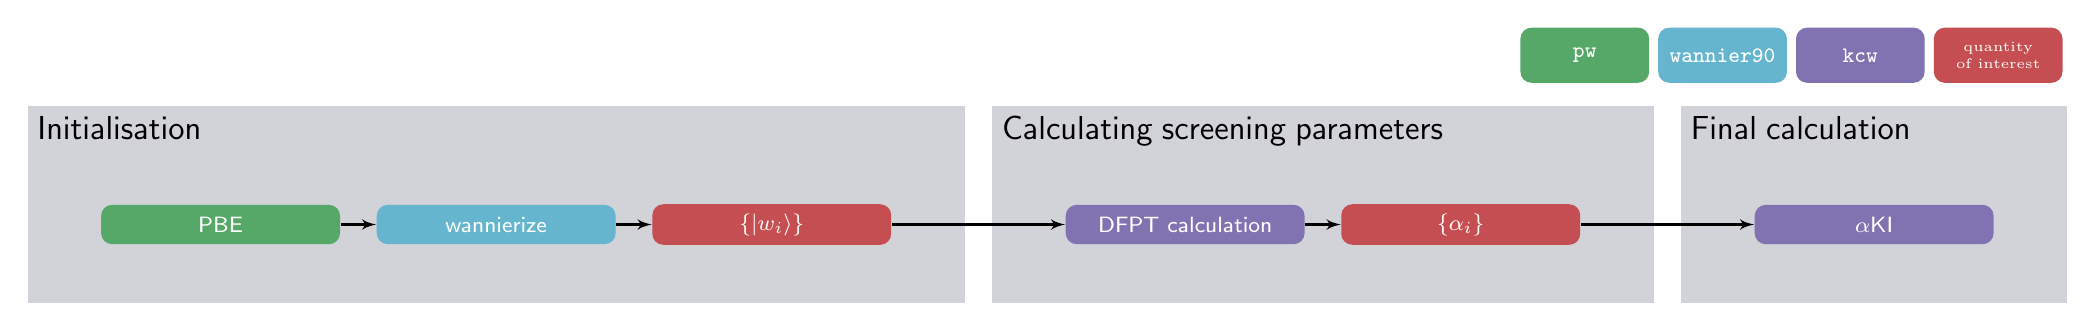
\begin{tikzpicture}[font=\tiny, x=3.5cm, y=1cm]
   \begin{pgfonlayer}{background}
      \fill [seaborn_bg_grey_dark] (-2.2,-1) rectangle (1.2,1.5);
      \node at (-2.2, 1.5) [default_text] {\large Initialisation};
      \fill [seaborn_bg_grey_dark] (1.3,-1) rectangle (3.7,1.5);
      \node at (1.3, 1.5) [default_text] {\large Calculating screening parameters};
      \fill [seaborn_bg_grey_dark] (3.8,-1) rectangle (5.2,1.5);
      \node at (3.8, 1.5) [default_text, text width=3.5cm] {\large Final calculation};
      % \fill [seaborn_bg_grey_dark] (8.1,-1) rectangle (9.1,1.5);
      % \node at (8.1, 1.5) [default_text, text width=3.5cm] {\large Postprocessing};
   \end{pgfonlayer}

   % Key
   \node at (3.45, 2.15) [pw, text width=1.4cm, minimum height=0.7cm] {\texttt{pw}};
   \node at (3.95, 2.15) [wannier90, text width=1.4cm, minimum height=0.7cm] {\texttt{wannier90}};
   \node at (4.45, 2.15) [kcw, text width=1.4cm, minimum height=0.7cm] {\texttt{kcw}};
   \node at (4.95, 2.15) [observable, text width=1.4cm, minimum height=0.7cm, font=\tiny] {quantity of interest};

   % Initialisation
   % Solids
   \node at (-1.5, 0) [pw] (pw PBE init) {PBE};
   \node at (-0.5, 0) [wannier90] (wannierize) {wannierize};
   \node at (0.5, 0) [observable] (unfold) {$\{\ket{w_i}\}$};
   \path [line] (pw PBE init) -- (wannierize);
   \path [line] (wannierize) -- (unfold);

   % Calculating screening parameters
   \node at (2, 0) [kcw] (KC screen) {DFPT calculation};
   \node at (3, 0) [observable] (alphas) {$\{\alpha_i\}$};
   \path [line] (unfold) -- (KC screen);
   \path [line] (KC screen) -- (alphas);

   % Final calc
   \node at (4.5, 0) [kcw] (KC ham) {$\alpha$KI};
   \path [line] (alphas) -- (KC ham);

\end{tikzpicture}
\end{frame}
\end{document}
